\documentclass{article}

%%%%%%%%%%%%%%%%%%%%%%%%%%%%%%%%%%%%%%%%%%%%%%%%%%%%%%%%%%%%%%%%%%%%%
%% Place any additional packages needed here.  Only include packages
%% which are essential, to avoid problems later. Do NOT use any
%% packages which require e-TeX (for example etoolbox): the e-TeX
%% extensions are not currently available on the ACS conversion
%% servers.
%%%%%%%%%%%%%%%%%%%%%%%%%%%%%%%%%%%%%%%%%%%%%%%%%%%%%%%%%%%%%%%%%%%%%
% \usepackage[version=3]{mhchem} % Formula subscripts using \ce{}
\usepackage{siunitx}
\usepackage{tabularx}
\usepackage{float}
\usepackage{booktabs}
\usepackage{amsmath}
\usepackage{amssymb}
\usepackage{amsfonts}
\usepackage{graphicx}
\usepackage{pdflscape}
\usepackage{geometry}
\geometry{a4paper, margin=1in}

\DeclareMathOperator*{\argmax}{arg\,max}
\DeclareMathOperator*{\argmin}{arg\,min}

\title{Supplementary information for Sensitivity test of Markov state models}

\begin{document}
\maketitle

\section{Summary of trial results}

\begin{table}[h]
    \centering
    \begin{tabular}{|l|c|}
       Number of  attempted trials   & 140 \\
       Number of trials with at least one successful bootstrap & 136 \\
       Smallest number of successful bootstrap trails & 88
    \end{tabular}
    \caption{\textsc{Trial statistics}. Results refers to a $\tau=\SI{41}{\nano\second}$ and the folding timescale ($t_{2}$).}
    \label{tab:summary_stats_1}
\end{table}


\begin{table}[h]
    \centering
    \begin{tabular}{l|l|l|c}
        Feature & Contact scheme & Distance transformation & Num. trials  \\
        \toprule
        Dihedrals & - & - & 20 \\
        Contact distances & $\alpha-$Carbon & Linear & 20 \\
        Contact distances & Closest-heavy & Linear & 20 \\
        Contact distances & $\alpha-$Carbon & Logistic & 36 \\
        Contact distances & Closest-heavy & Logistic & 40 \\
    \end{tabular}
    \caption{\textsc{Trial statistics per feature}. Results refers to a $\tau=\SI{41}{\nano\second}$ and the folding timescale ($t_{2}$). `Num. trials' refers to the number of trials with at least one successful bootstrap.}
    \label{tab:summary_stats_2}
\end{table}

\begin{figure}
    \centering
    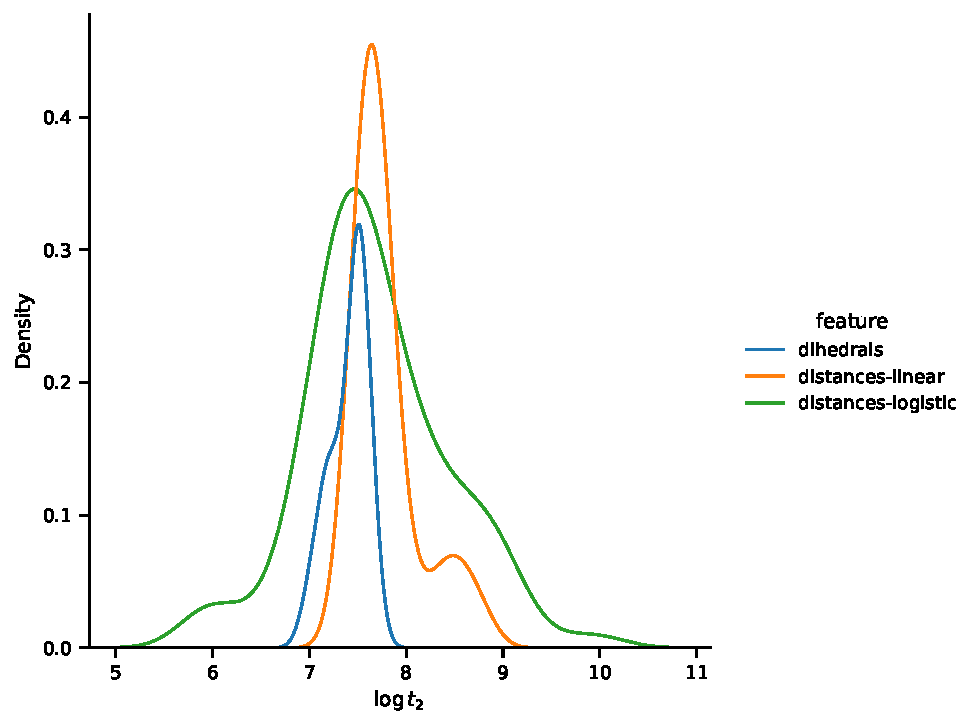
\includegraphics{figures/timescale_dist_summary.pdf}
    \caption{\textsc{Distribution of the folding timescale}. The log of $t_2$, for each feature. }
    \label{fig:ts_distribution}
\end{figure}

\section{Choosing the Markov lag time}

The Markov lag time was estimated from the \num{136} successful trials.  

\begin{figure}[h]
    \centering
    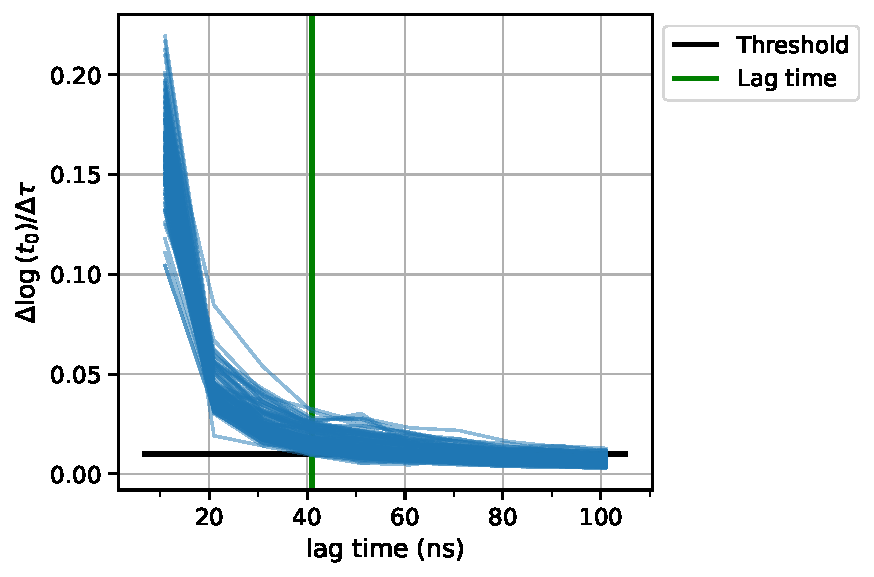
\includegraphics[width=0.8\textwidth]{figures/BBA_timescale_gradient.pdf}
    \caption{\textsc{Gradient of $t_{2}$ with respect to the Markov lag time.} Each is calculated according to equation~\ref{eqn:choose_lag_1}.  The black horizontal line is the gradient threshold ($\log{1.01}$) and the vertical green line is the selected lag time, selected according to equation~\ref{eqn:choose_lag_2}. }
    \label{fig:choose_lag}
\end{figure}

\section{How does the number of scored processes affect model selection?}

\begin{figure}
    \centering
    \includegraphics[width=1.0\textwidth]{figures/vampeq_rank_vs_proc_pairplot.pdf}
    \caption{\textsc{Pair plot of $\operatorname{VAMP2}_{eq}(k)$ rank with different numbers of scored processes}. The panel at position $(0,1)$ plots the rank according to$\operatorname{VAMP2}_{eq}(2)$ against the  rank according to$\operatorname{VAMP2}_{eq}(3)$, and similarly for other positions. This }
    \label{fig:vampeq_rank_vs_proc_pairplot}
\end{figure}

\section{How does the lag time affect model selection?}

\begin{figure}
    \centering
    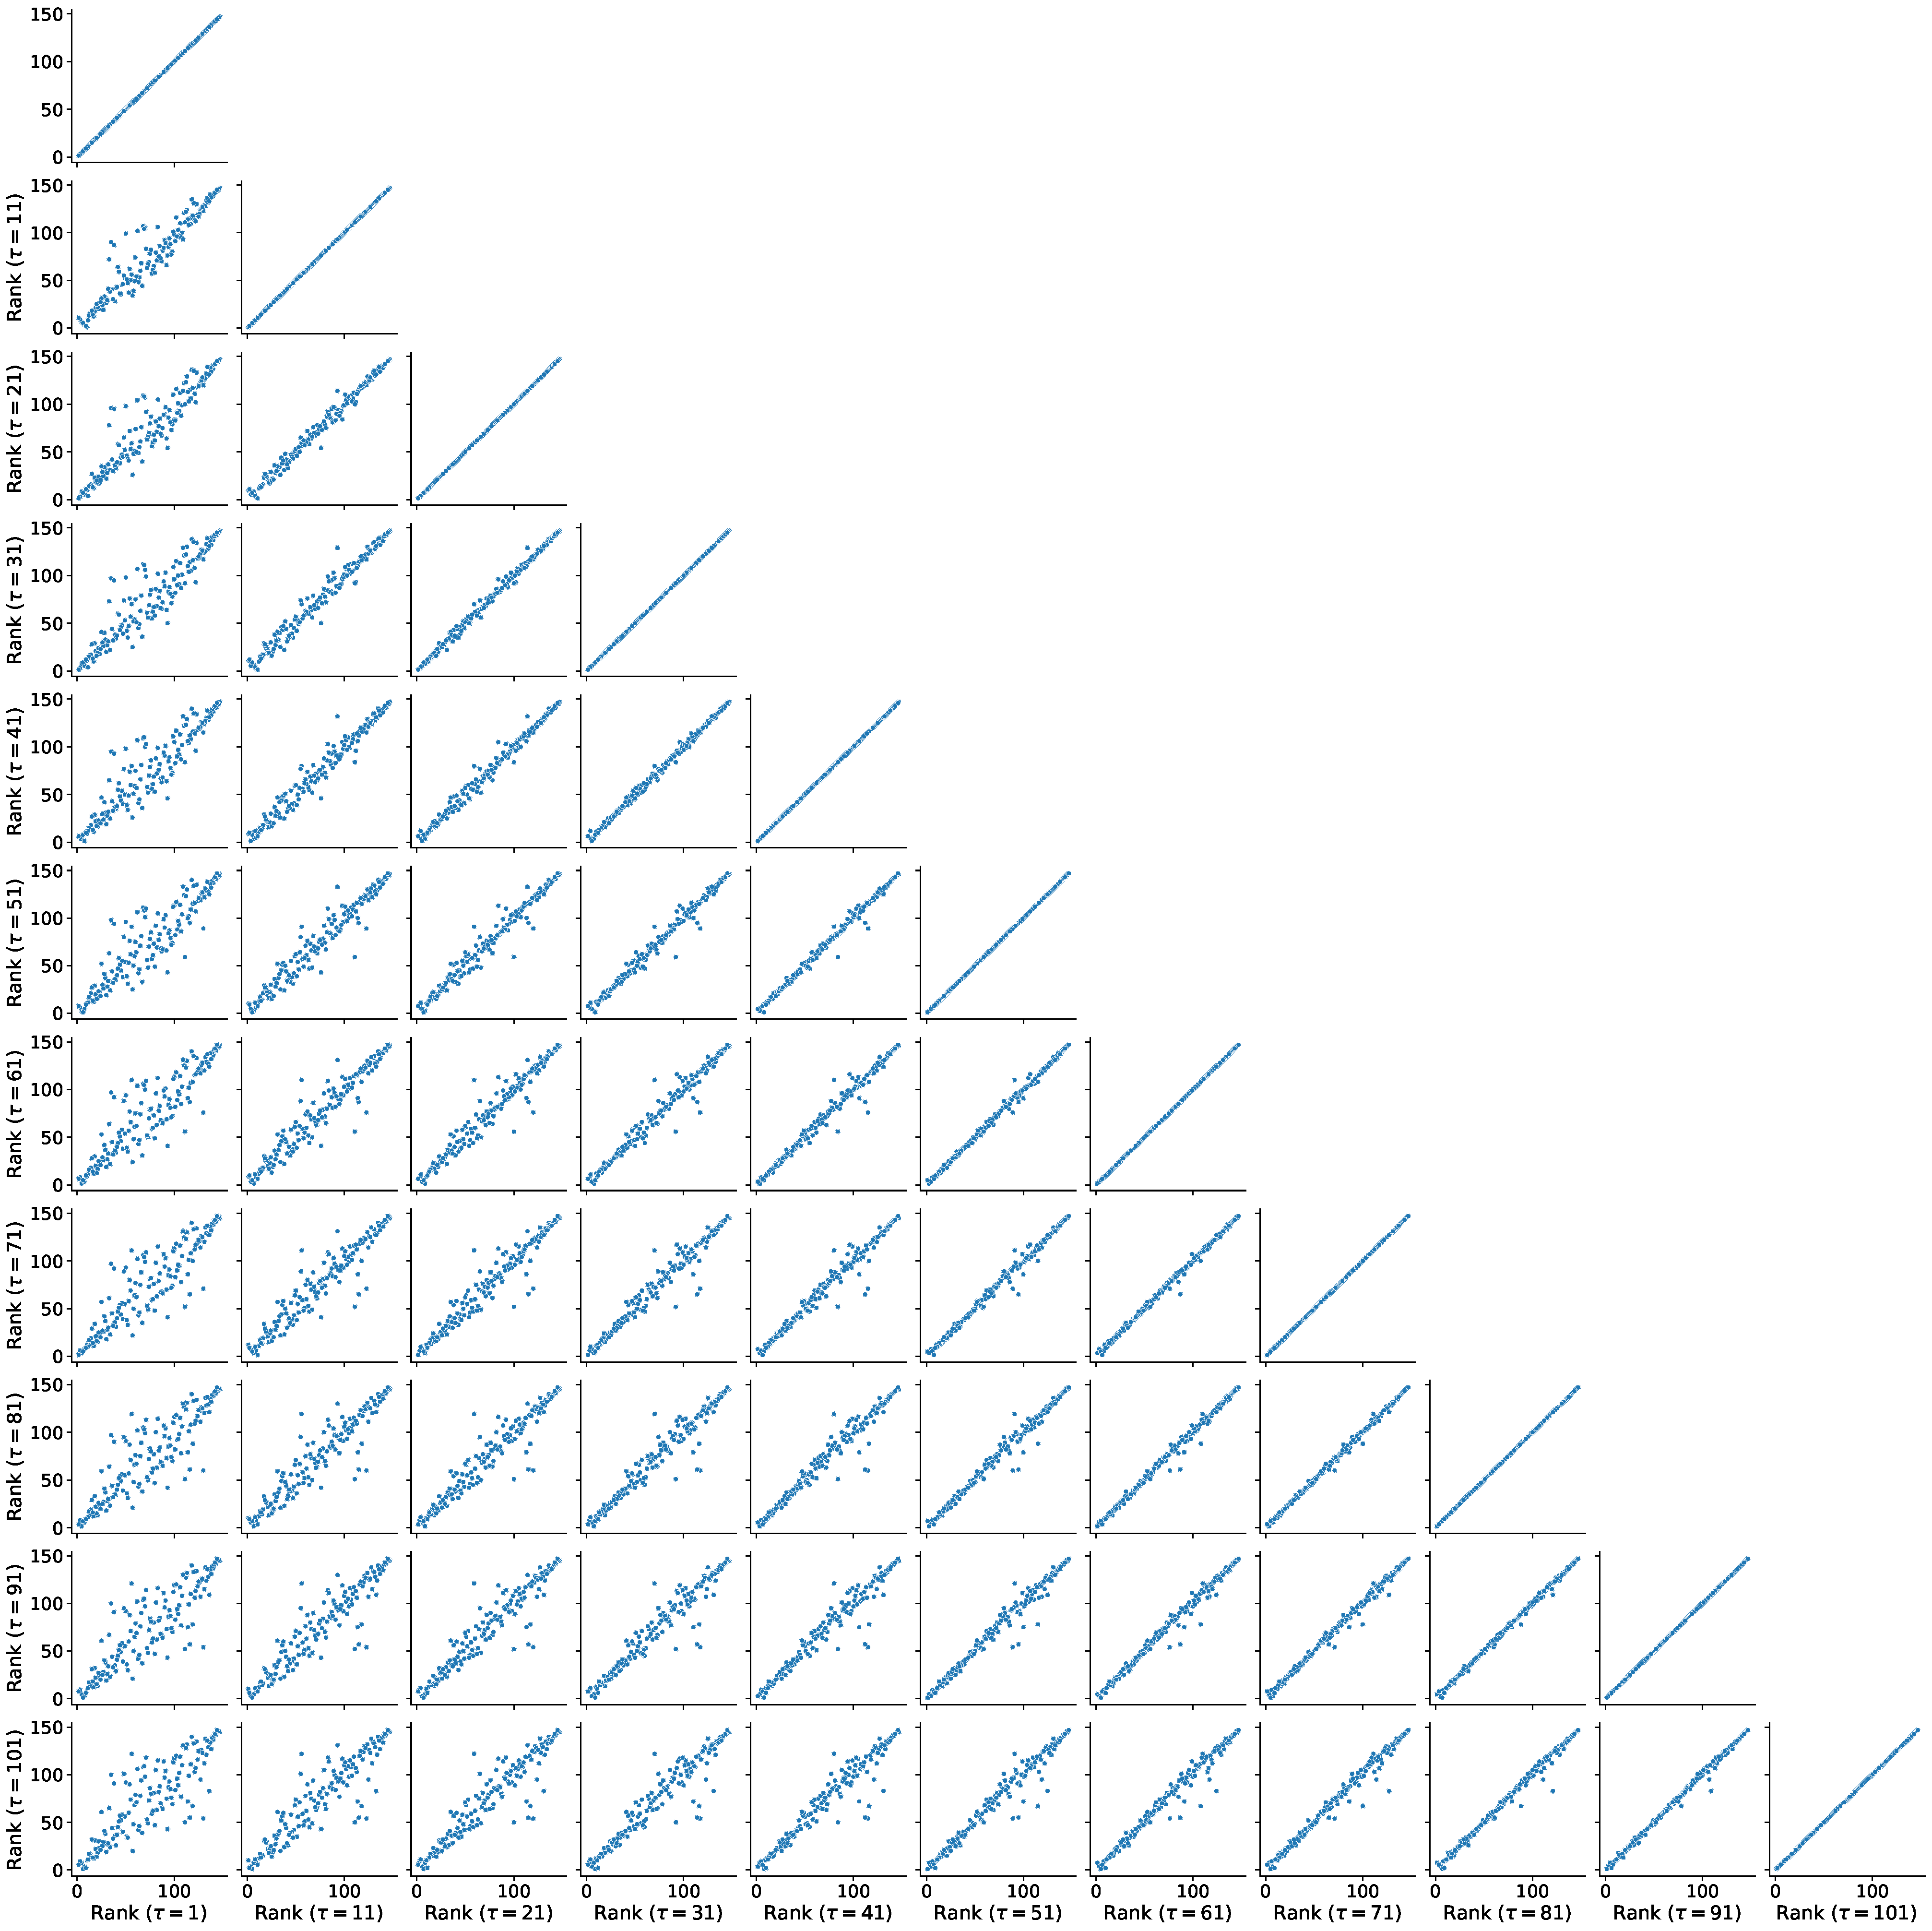
\includegraphics[width=1.0\textwidth]{figures/vampeq_rank_vs_lag_pairplot_k2.pdf}
    \caption{\textsc{Pair plot of $\operatorname{VAMP2}_{eq}(k=2)$ rank with different lag times.} The panel at position $(0,1)$ plots the rank according to$\operatorname{VAMP2}_{eq}(2)$ against the  rank according to$\operatorname{VAMP2}_{eq}(3)$, and similarly for other positions. This }
    \label{fig:vampeq2_rank_vs_lag_pairplot}
\end{figure}


\begin{figure}
    \centering
    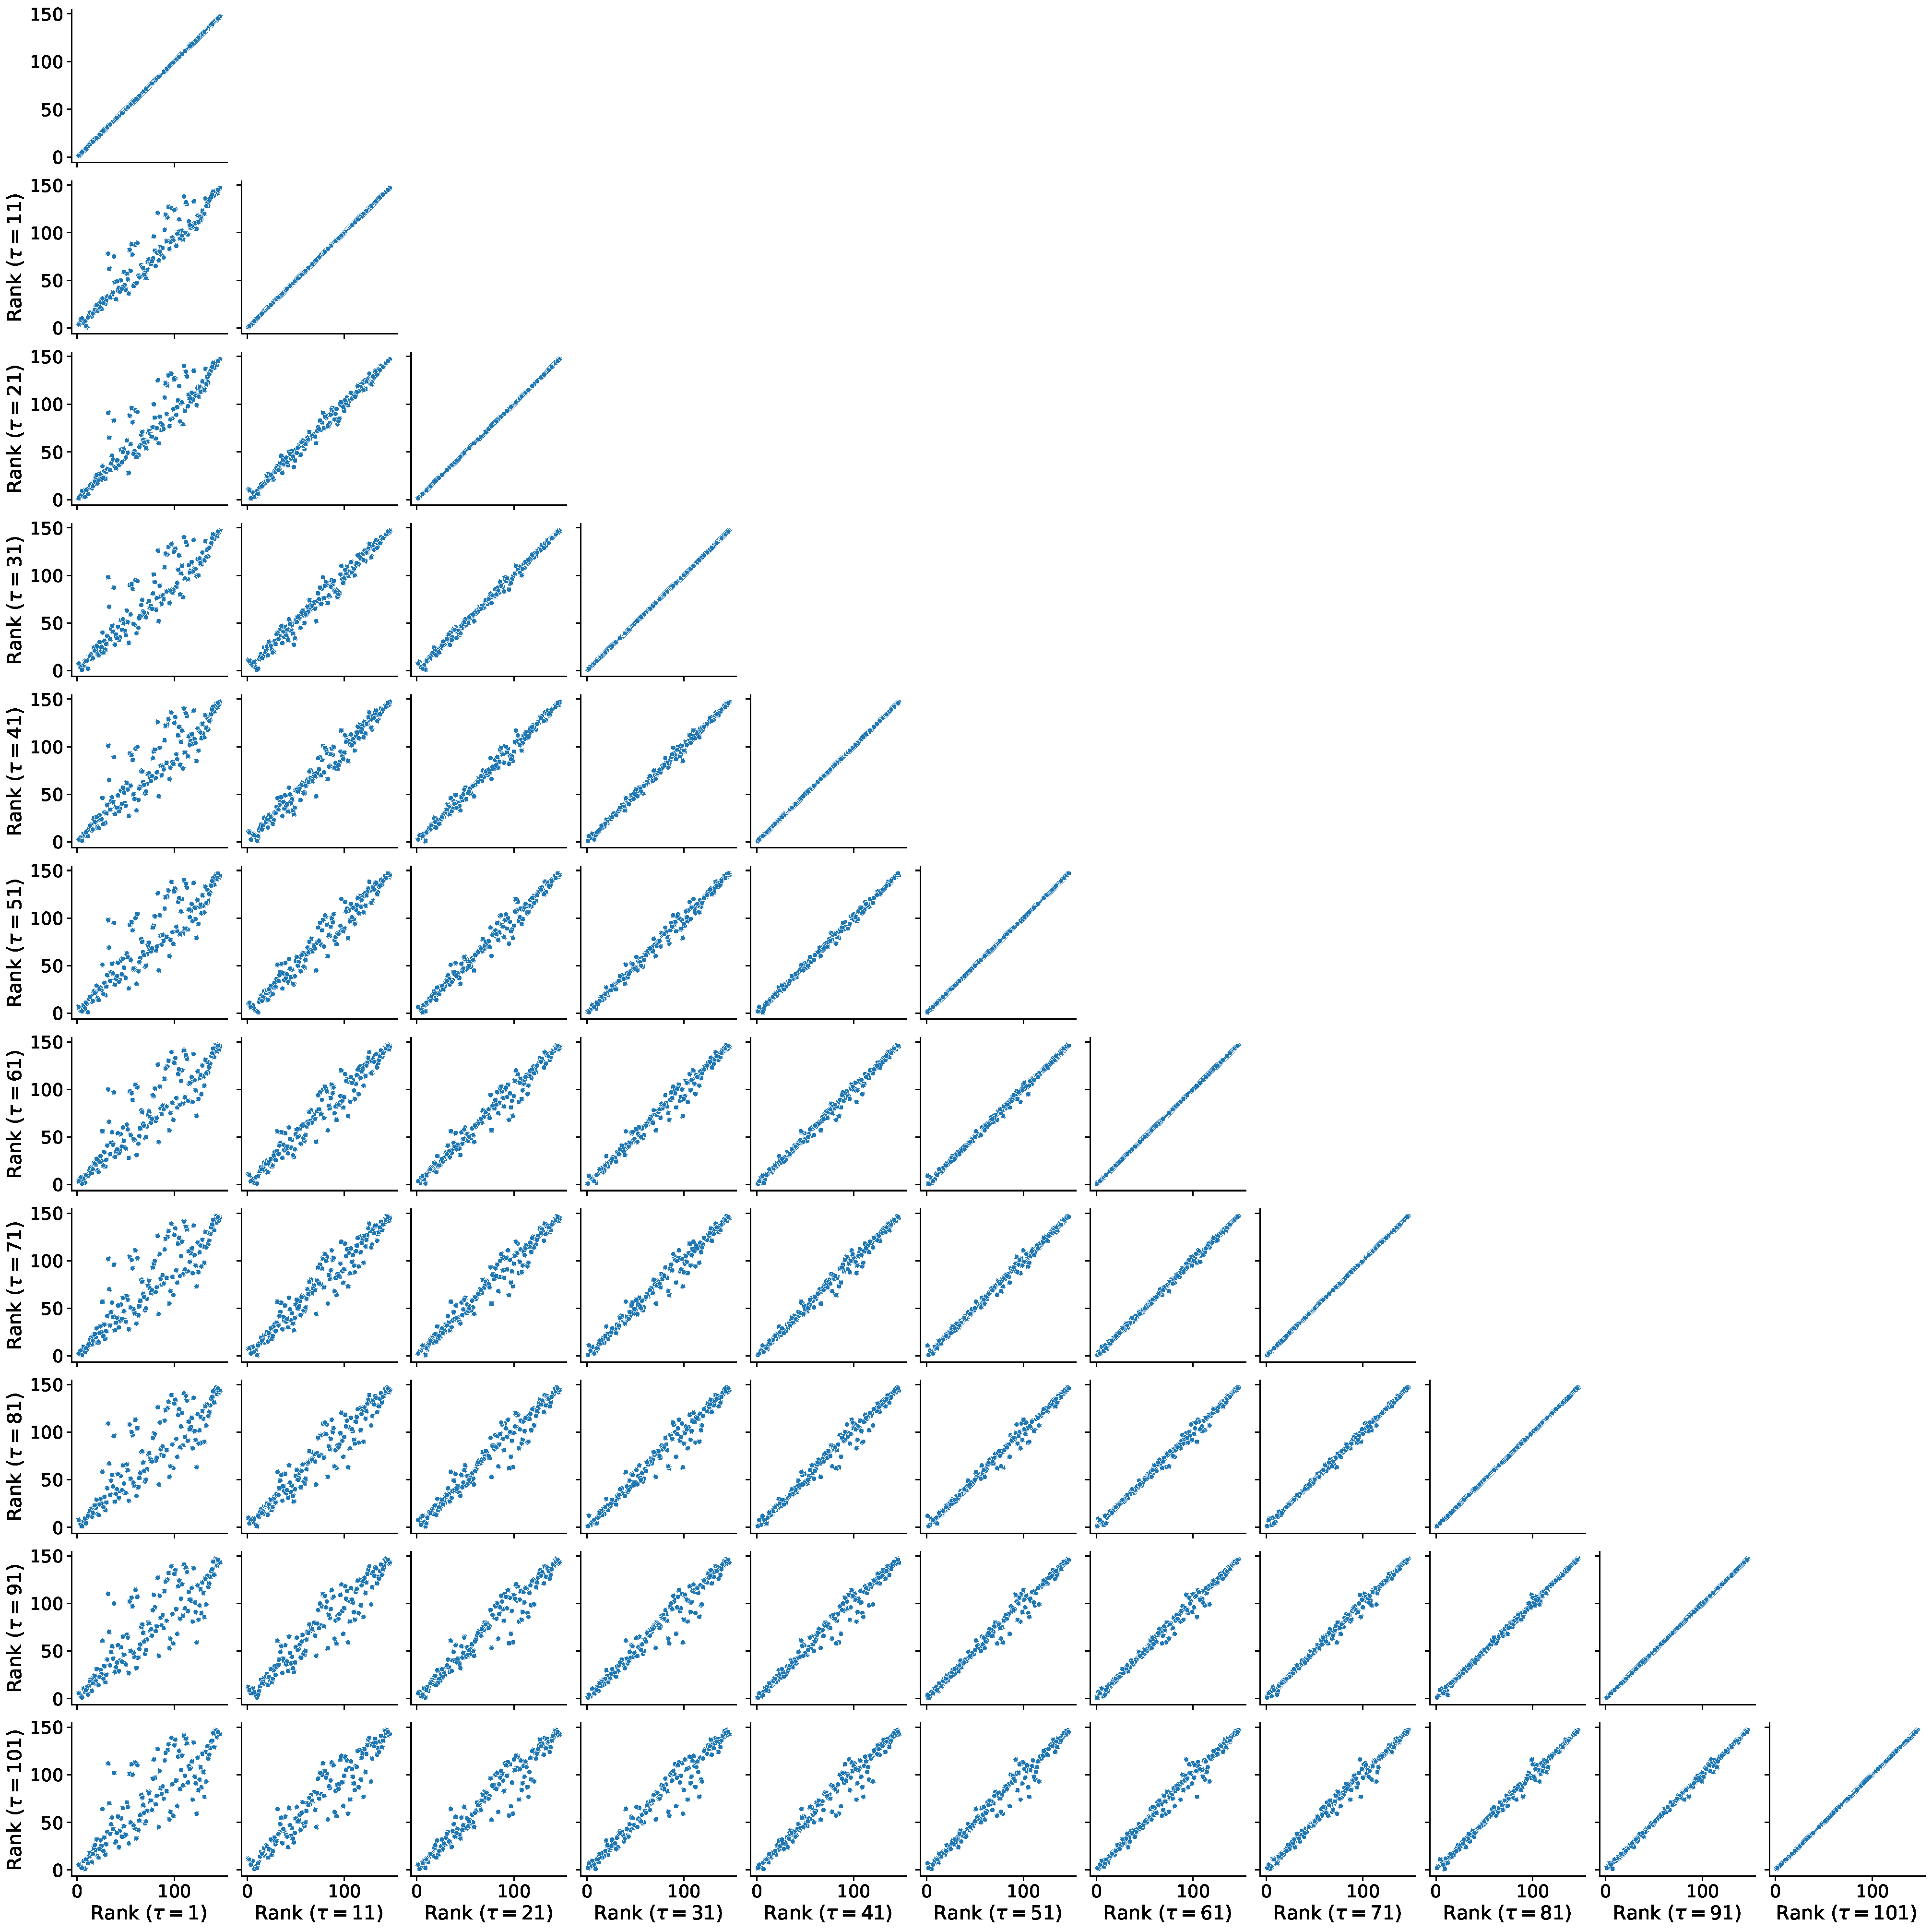
\includegraphics[width=1.0\textwidth]{figures/vampeq_rank_vs_lag_pairplot_k3.pdf}
    \caption{\textsc{Pair plot of $\operatorname{VAMP2}_{eq}(k=3)$ rank with different lag times.} The panel at position $(0,1)$ plots the rank according to$\operatorname{VAMP2}_{eq}(2)$ against the  rank according to$\operatorname{VAMP2}_{eq}(3)$, and similarly for other positions. This }
    \label{fig:vampeq3_rank_vs_lag_pairplot}
\end{figure}

\begin{figure}
    \centering
    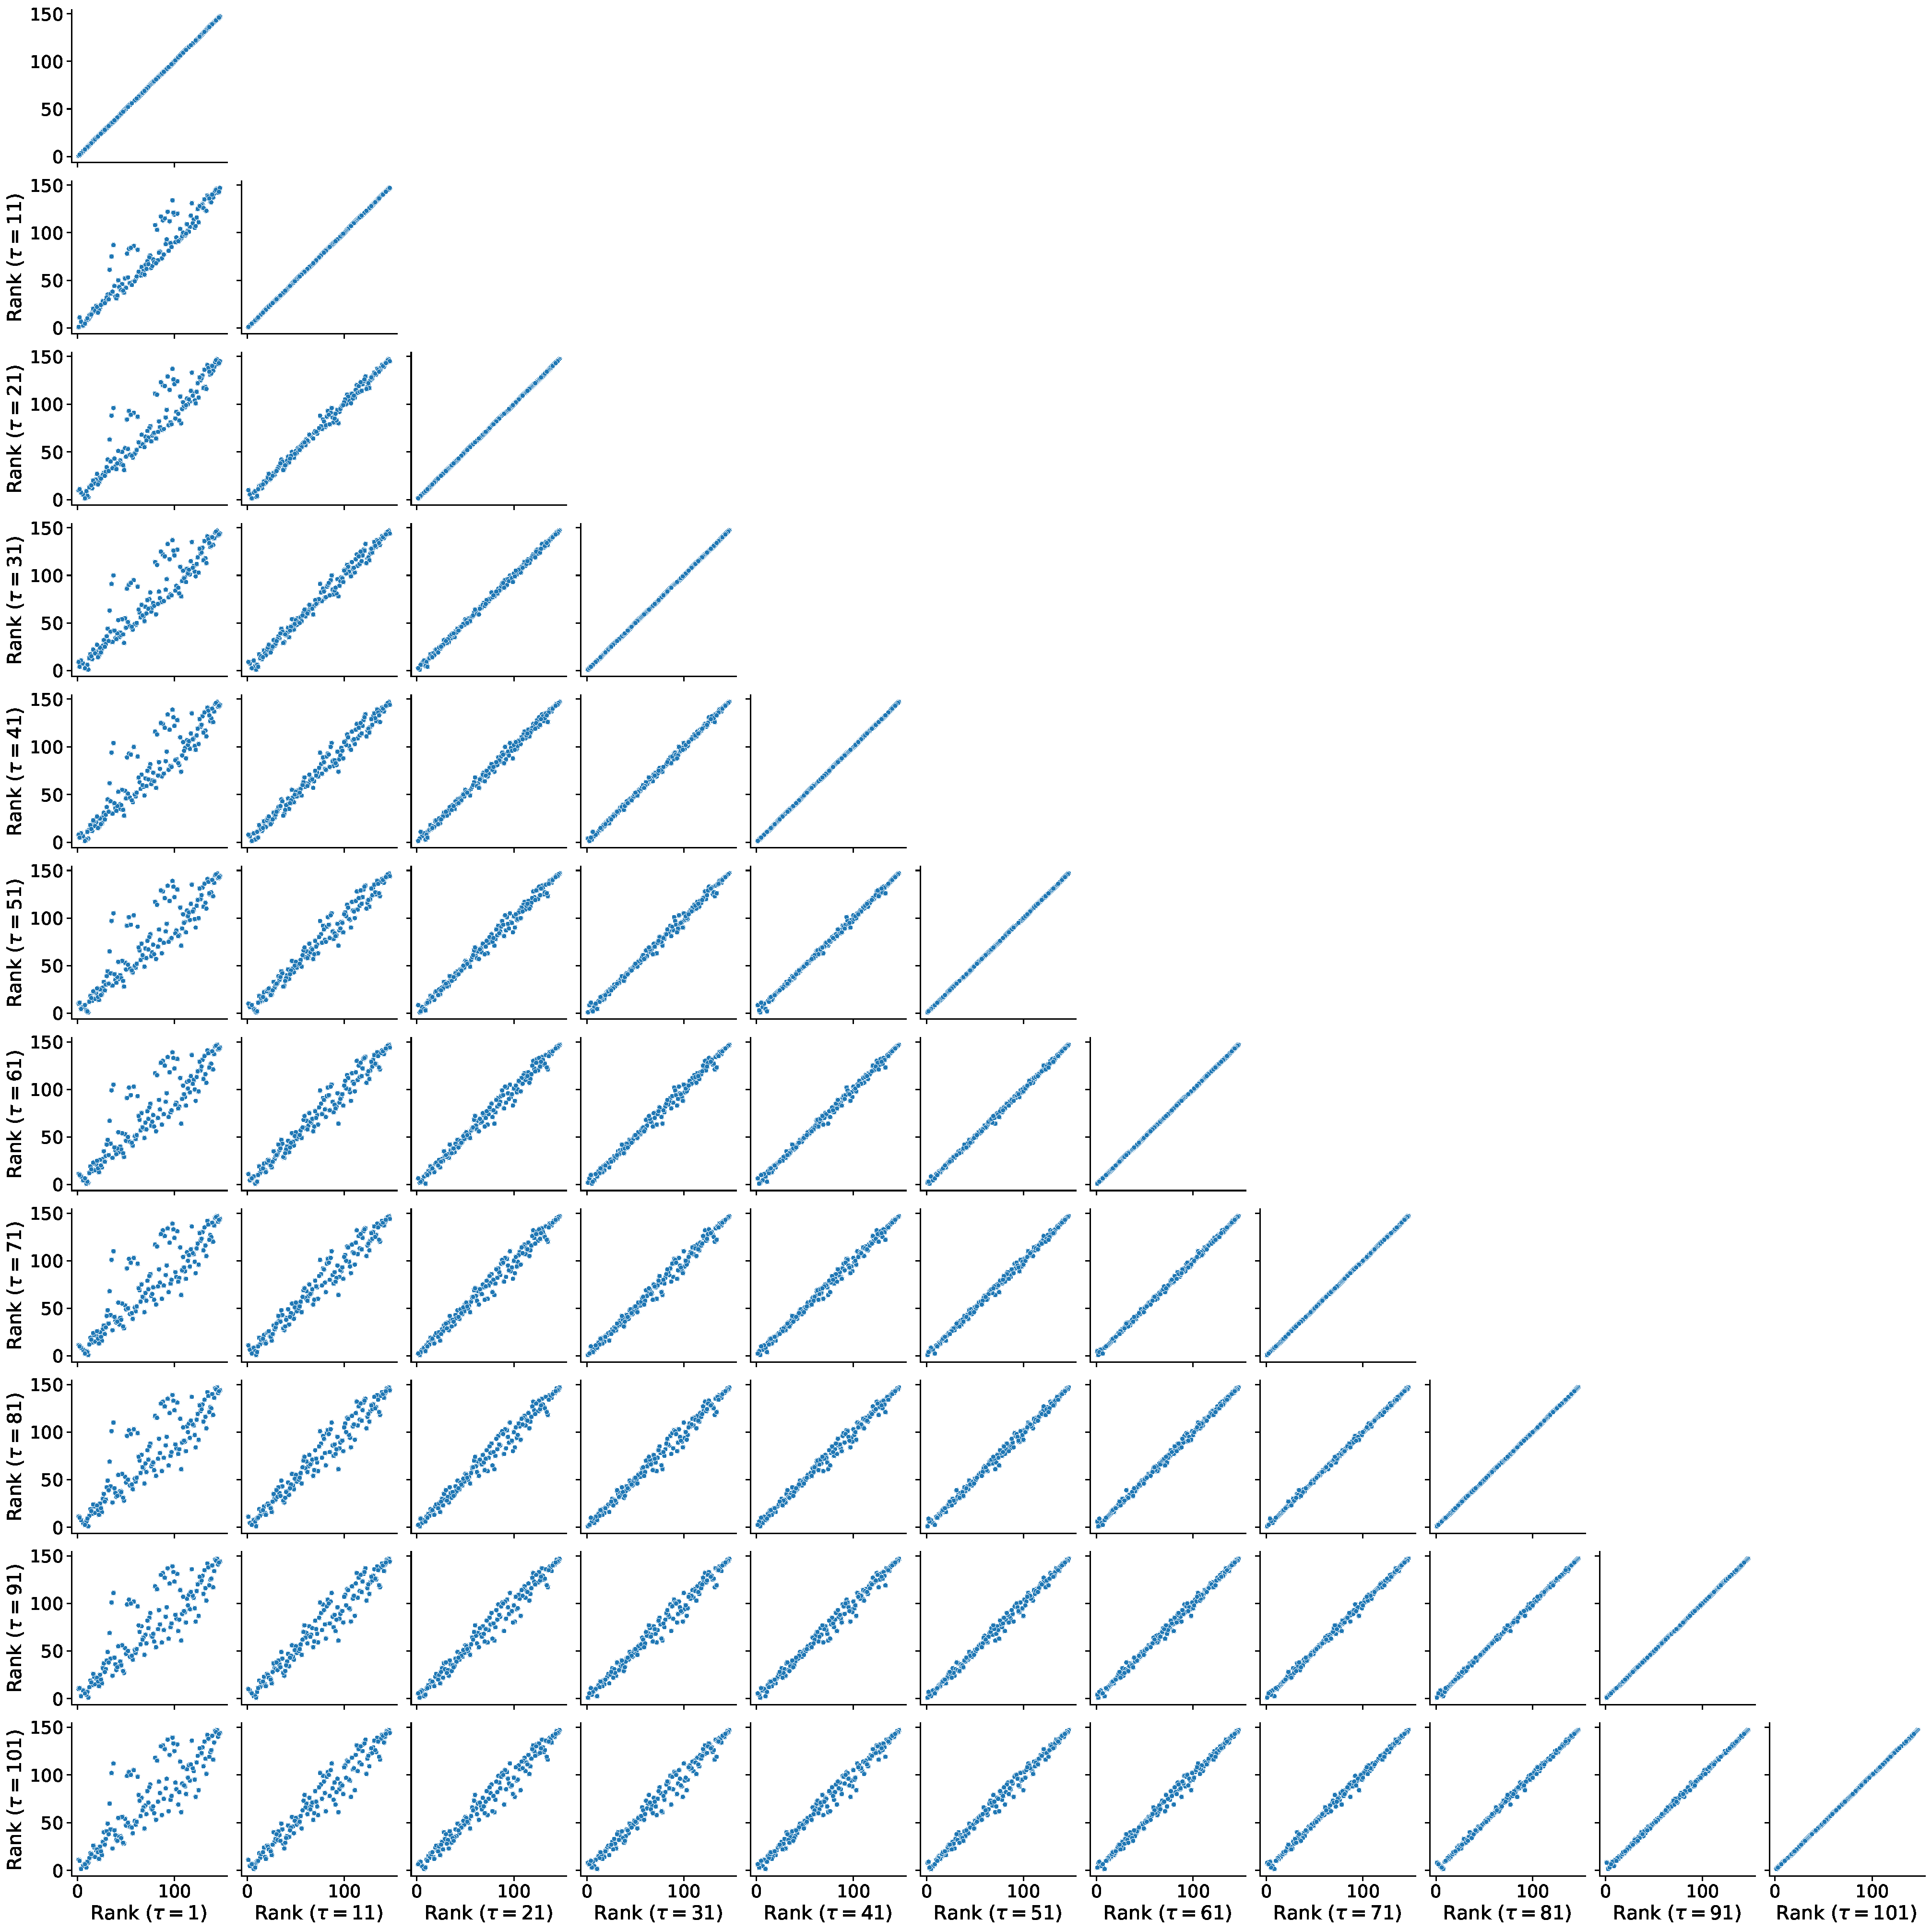
\includegraphics[width=1.0\textwidth]{figures/vampeq_rank_vs_lag_pairplot_k5.pdf}
    \caption{\textsc{Pair plot of $\operatorname{VAMP2}_{eq}(k=3)$ rank with different lag times.} The panel at position $(0,1)$ plots the rank according to$\operatorname{VAMP2}_{eq}(2)$ against the  rank according to$\operatorname{VAMP2}_{eq}(3)$, and similarly for other positions. This }
    \label{fig:vampeq5_rank_vs_lag_pairplot}
\end{figure}

\begin{figure}
    \centering
    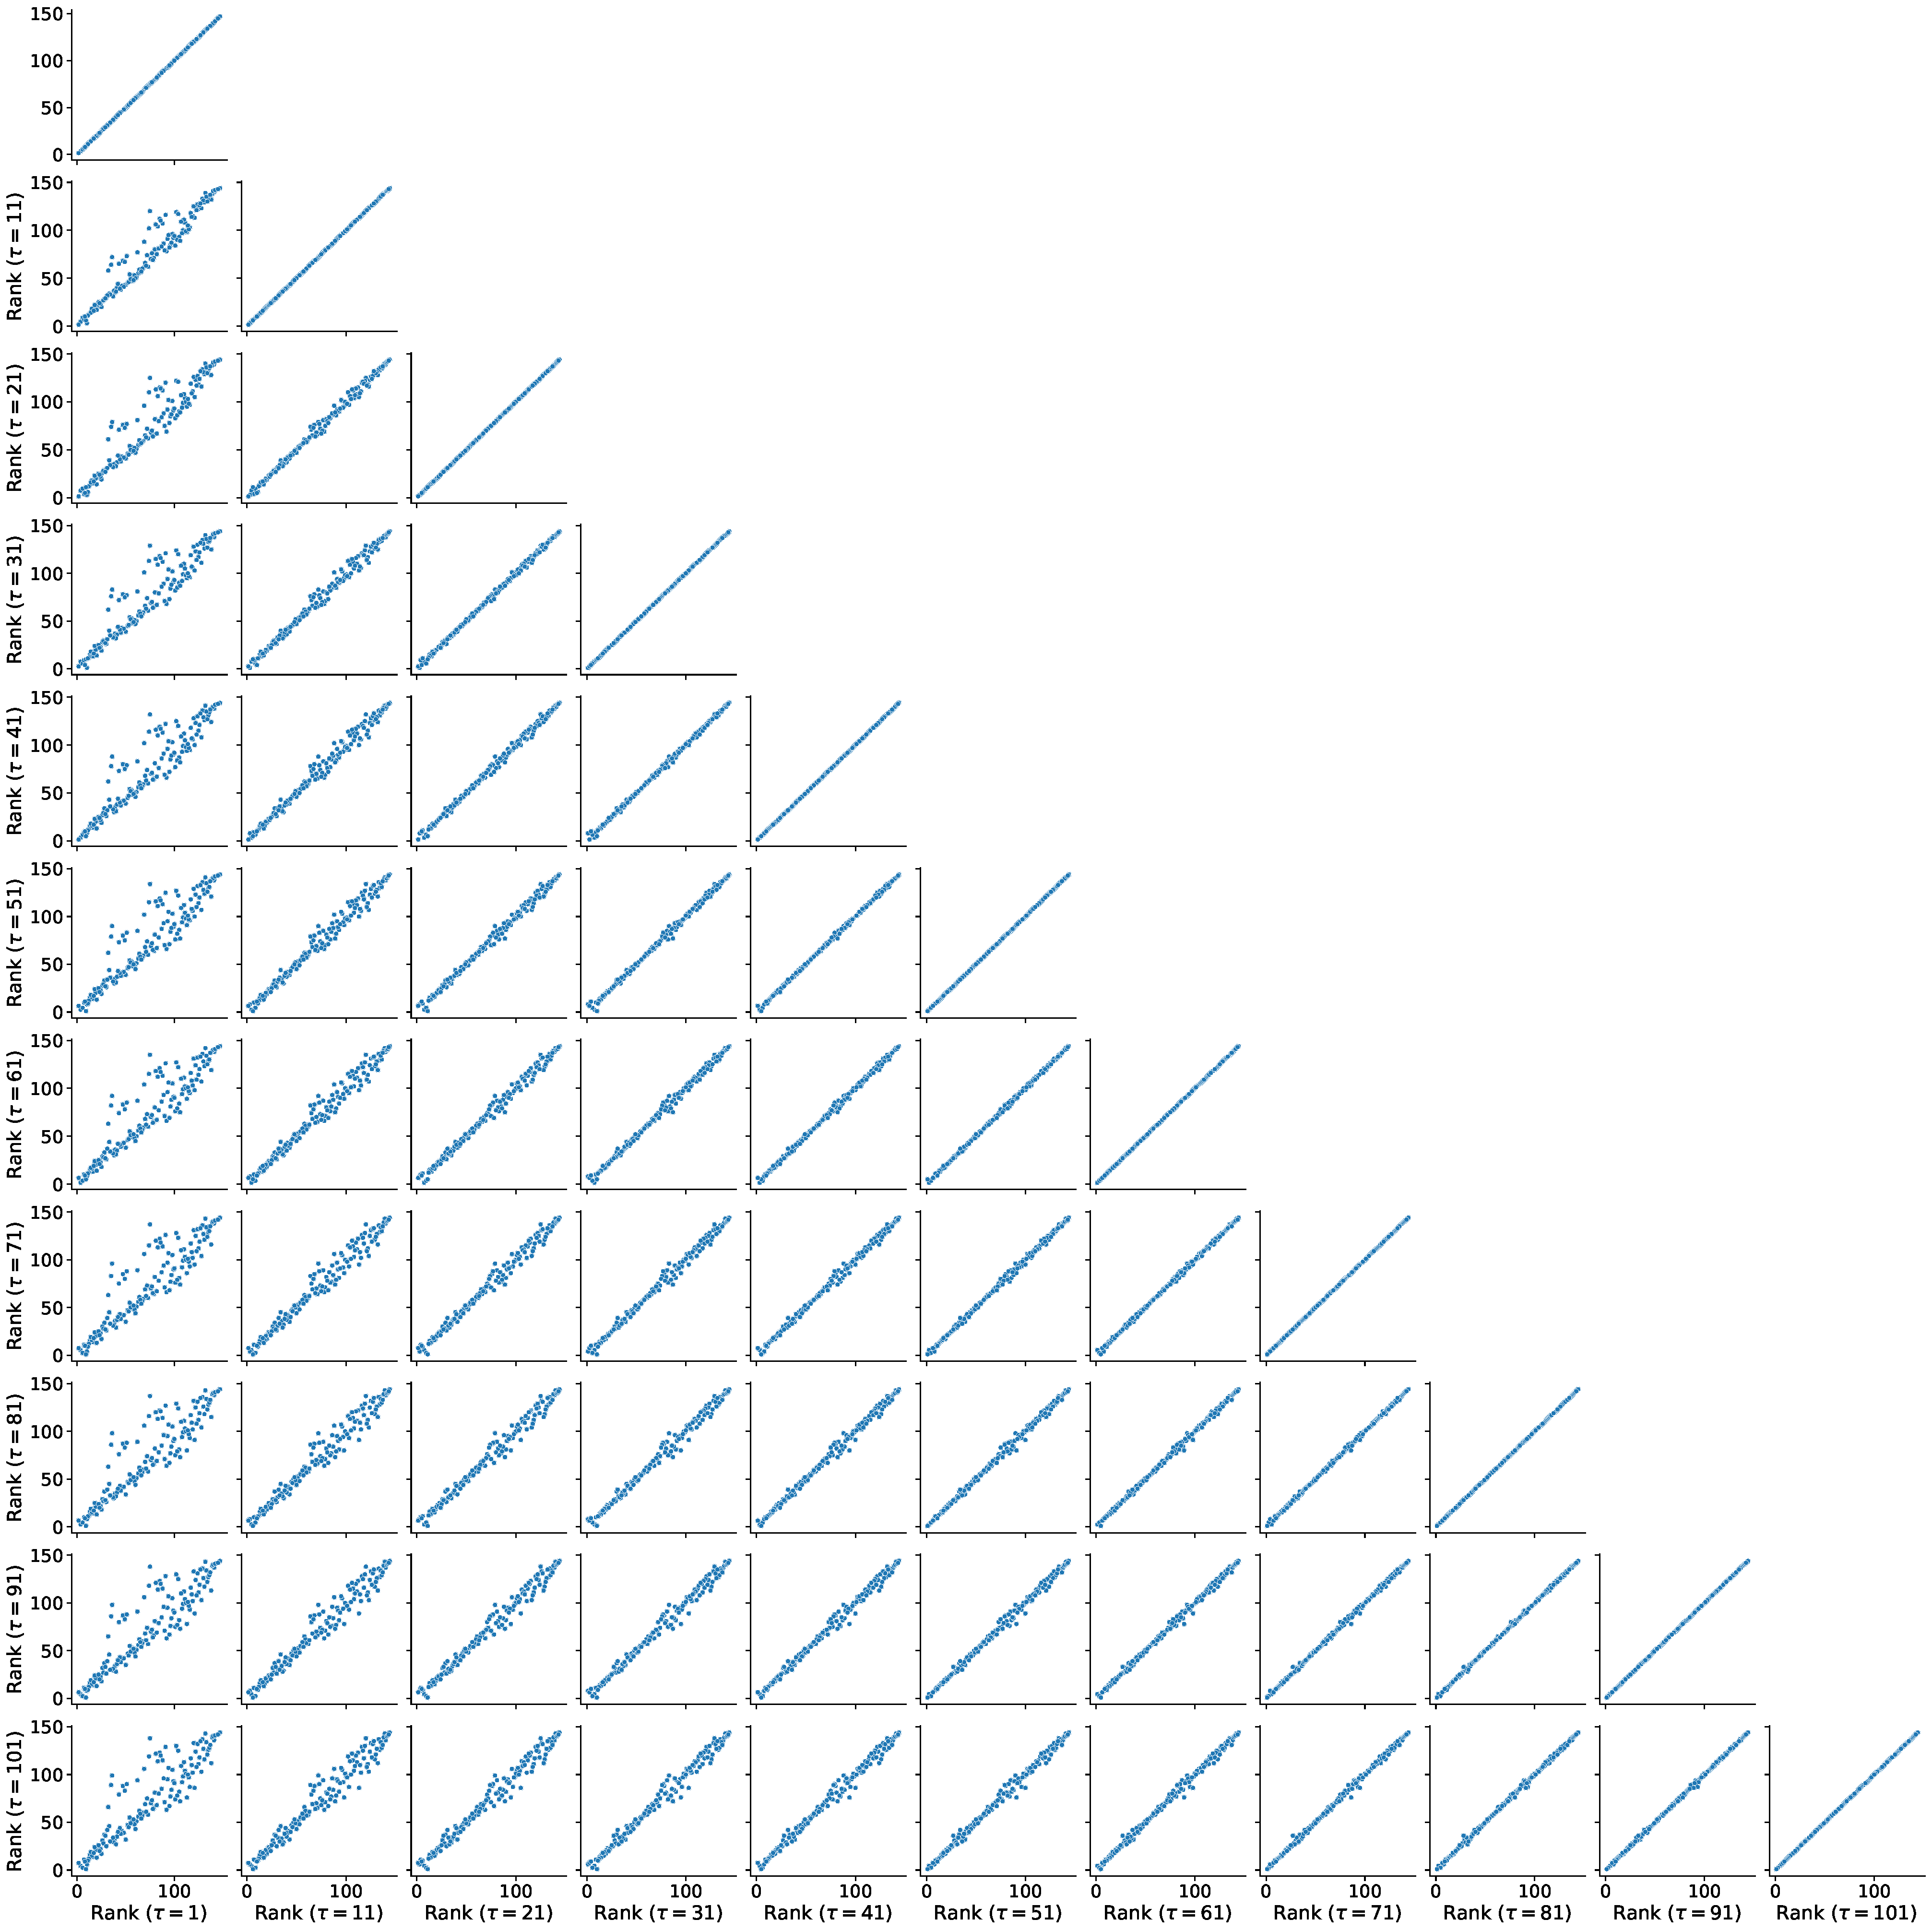
\includegraphics[width=1.0\textwidth]{figures/vampeq_rank_vs_lag_pairplot_k10.pdf}
    \caption{\textsc{Pair plot of $\operatorname{VAMP2}_{eq}(k=5)$ rank with different lag times.} The panel at position $(0,1)$ plots the rank according to$\operatorname{VAMP2}_{eq}(2)$ against the  rank according to$\operatorname{VAMP2}_{eq}(3)$, and similarly for other positions. This }
    \label{fig:vampeq10_rank_vs_lag_pairplot}
\end{figure}

\section{Modelling the hyperparameter response surface}\label{sec:response_surface_fitting}


\begin{figure}[h]
    \centering
    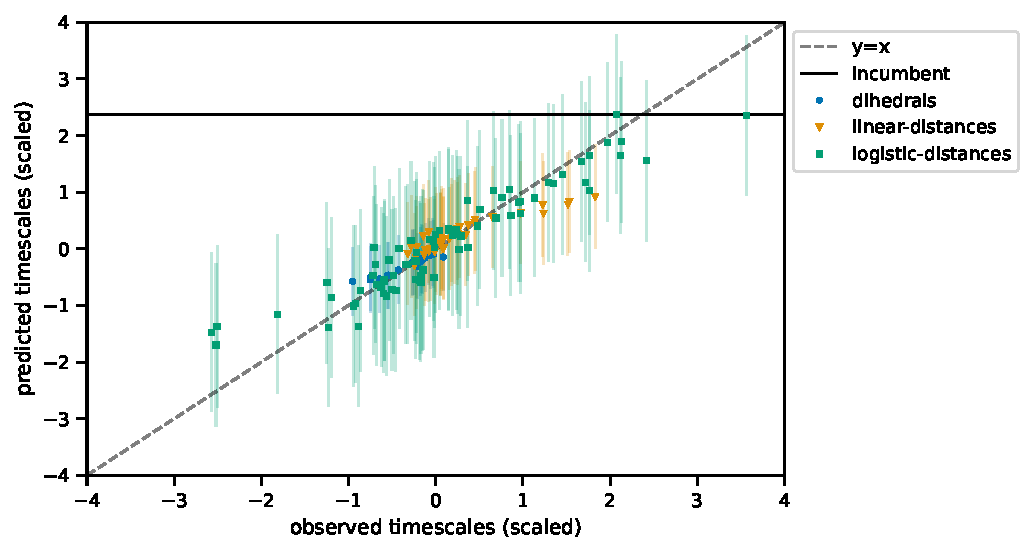
\includegraphics[width=0.8\textwidth]{figures/response_surface_predictions_ts.pdf}
    \caption{Response surface predictions. The timescales are modelled (after a log-transform and scaling) as a Gaussian process, separately for each feature. The predictions and error bars are the $(\mu, 2\sigma)$ of the Gaussian process. The incumbent is the largest mean predicted value. }
    \label{fig:response_surface}
\end{figure}

How the models were fit to the data. 

\section{Estimating the hyperparameter relevance}\label{sec:hp_relevance_calc}

These were chosen so as to maximize the expected improvement, i.e., the figure plots $y=f(s, c, d^{*}, m^{*}, \tau^{*}, n^{*})$ where $s^{*}, c^{*}, d^{*}, m^{*}, \tau^{*}, n^{*} = \argmax \left [f(s, c, d, m, \tau,n)\right]$.


\begin{figure}
    \centering
    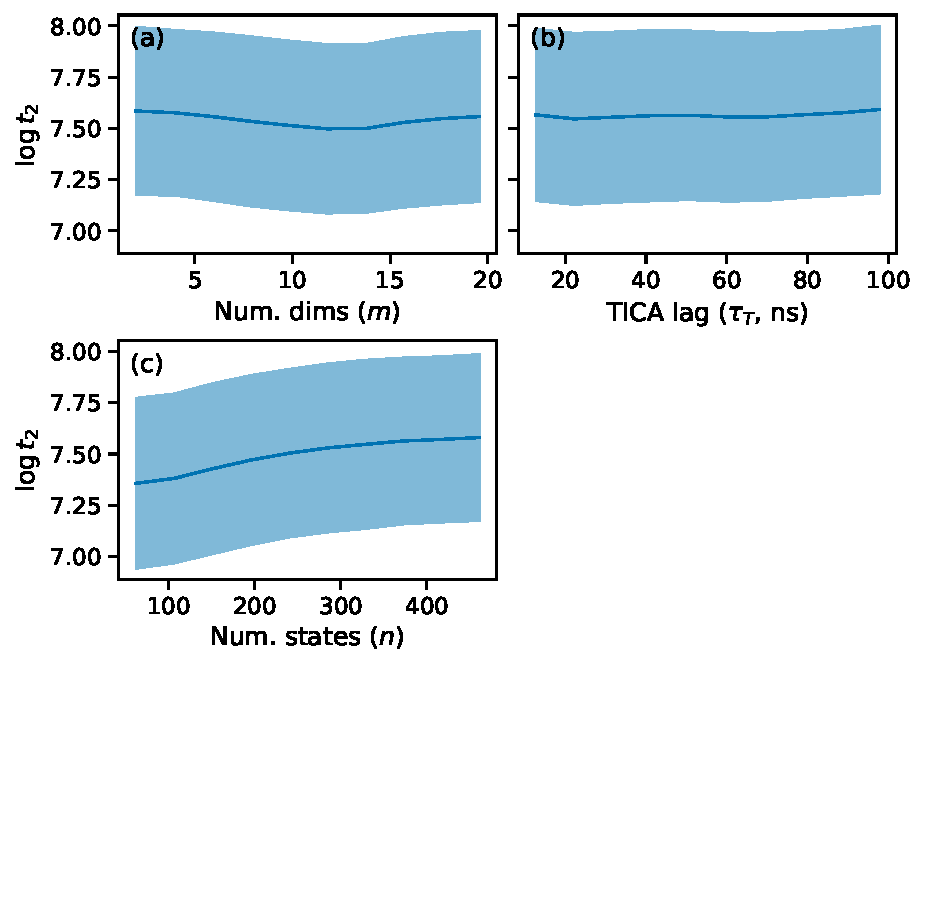
\includegraphics[width=0.8\textwidth, trim={0, 4cm, 0, 0}, clip]{figures/response_surface_marginal_dihedrals_None_ts.pdf}
    \caption{\textsc{Timescale response surface dihedrals feature}. The solid line is the mean of the Gaussian process and the shaded area is $\pm 2\sigma$. Panel (a) shows the response surface as a function of the number of $m$, the number TICA dimensions. The remaining hyperparameters are fixed at the values at the maximum of the response surface. i.e., $\log{t_2}=f(m, \tau^{*}, n^{*})$ where $m^{*}, \tau^{*}, n^{*} = \argmax \left [f( m, \tau,n)\right]$. Panels (b) and (c) are similar but as functions of the TICA lag time ($
    \tau_{T}$) and number of microstates ($n$) respectively.}
    \label{fig:repsonse_diheds}
\end{figure}

\begin{figure}
    \centering
    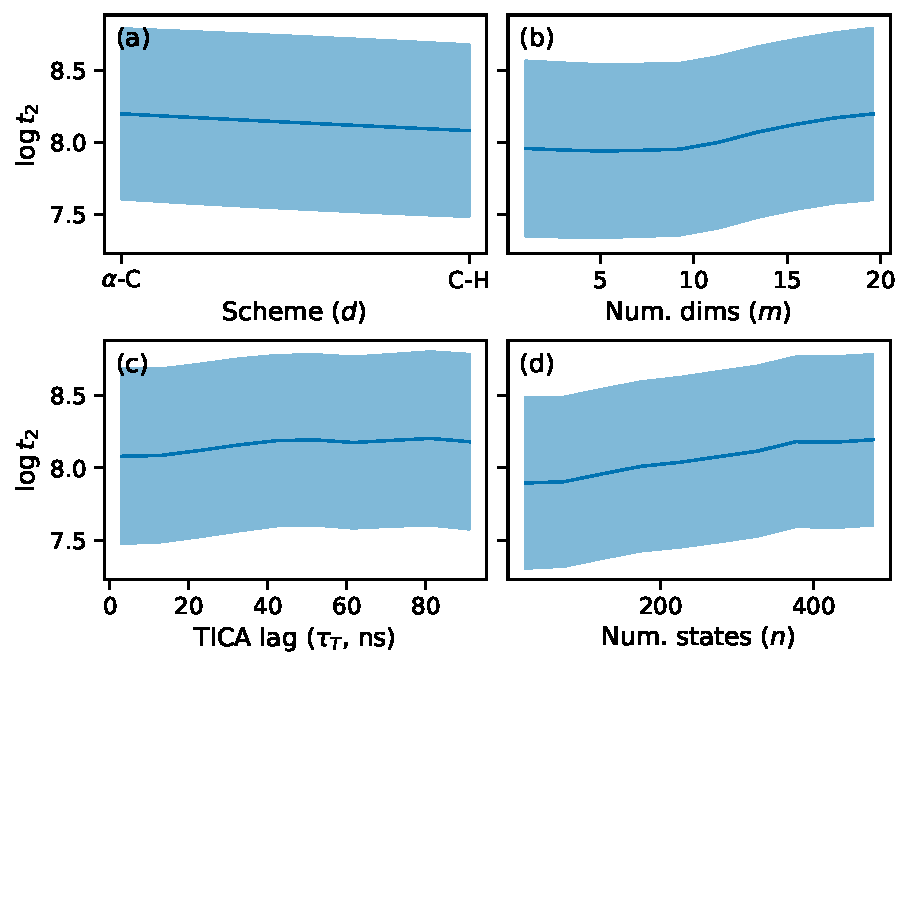
\includegraphics[width=0.8\textwidth, trim={0, 4cm, 0, 0}, clip]{figures/response_surface_marginal_distances_linear_ts.pdf}
    
    \caption{\textsc{Timescale response surface for distances feature}. The solid line is the mean of the Gaussian process and the shaded area is $\pm 2\sigma$. Panel (a) shows the response surface as a function of the number of $d$, the type of contact distance. The remaining hyperparameters are fixed at the values at the maximum of the response surface. i.e., $\log{t_2}=f(d, m^{*}, \tau^{*}, n^{*})$ where $d^{*}, m^{*}, \tau^{*}, n^{*} = \argmax \left [f(d,  m, \tau,n)\right]$. Panels (b), (c) and (d) are similar but as functions of the number of TICA dimensions ($m$), the TICA lag time ($\tau_{T}$) and number of microstates ($n$) respectively.}
    \label{fig:repsonse_dist}
\end{figure}


\begin{figure}
    \centering
    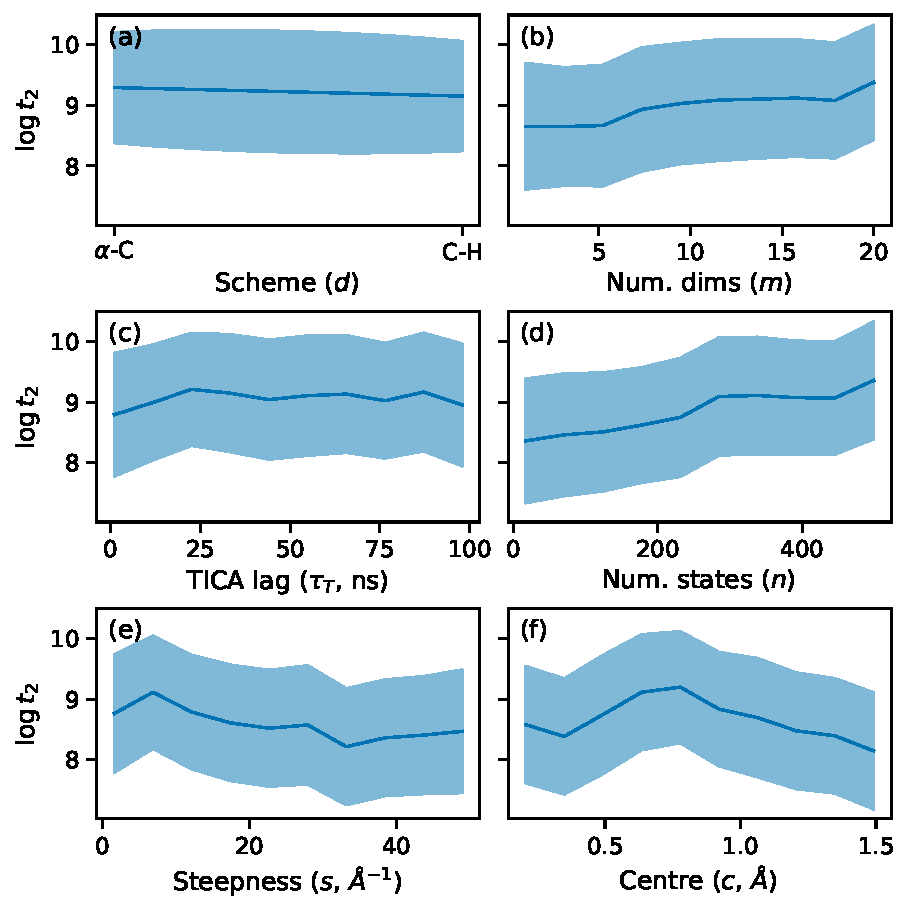
\includegraphics[width=0.8\textwidth]{figures/response_surface_marginal_distances_logistic_ts.pdf}
    \caption{\textsc{Timescale response surface for logistic distance feature}. The solid line is the mean of the Gaussian process and the shaded area is $\pm 2\sigma$. Panel (a) shows the response surface as a function of the number of $d$, the type of contact distance. The remaining hyperparameters are fixed at the values at the maximum of the response surface. i.e., $\log{t_2}=f(d, m^{*}, \tau^{*}, n^{*}, s^{*}), c^{*})$ where $d^{*}, m^{*}, \tau^{*}, n^{*}, s^{*}, c^{*} = \argmax \left [f(d,  m, \tau,n, s, c)\right]$. Panels (b), (c), (d), (e) and (f) are similar but as functions of the number of TICA dimensions ($m$), the TICA lag time ($\tau_{T}$), number of microstates ($n$), logistic steepness ($s$) and logistic center ($c$) respectively.}
    \label{fig:repsonse_logistic}
\end{figure}


Details on the bootstrapping process


\section{Bayesian Optimisation}

\begin{figure}
    \centering
    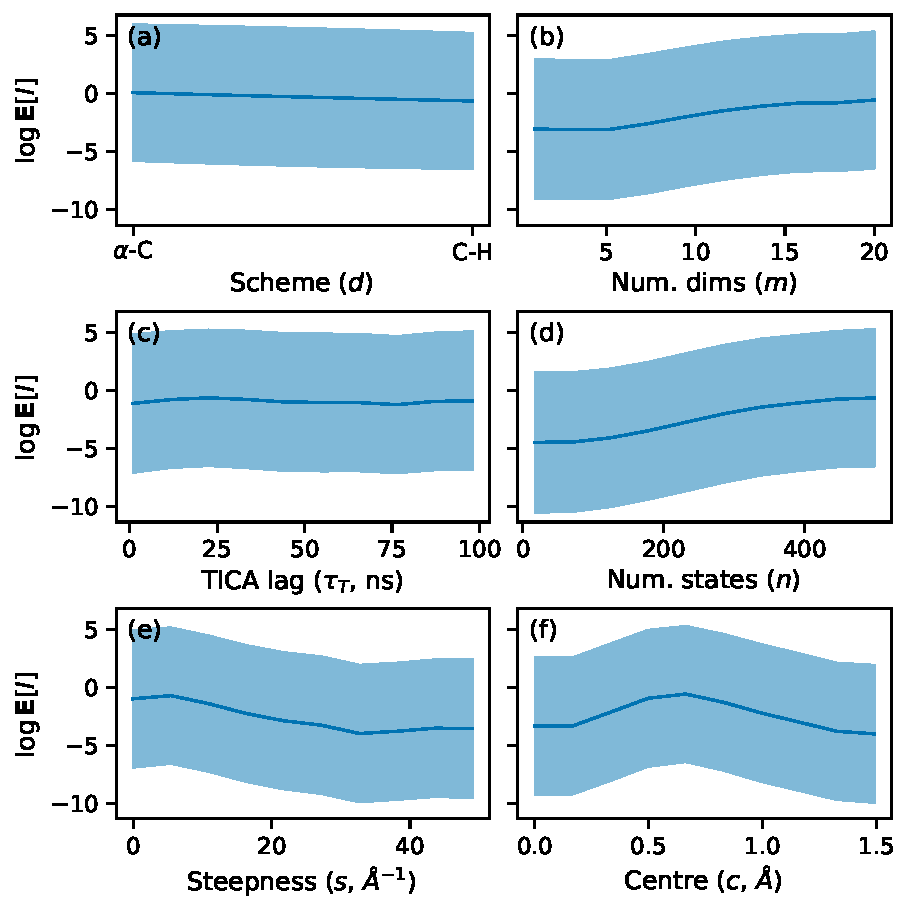
\includegraphics[width=0.8\textwidth]{figures/response_surface_marginal_distances_logistic_ei.pdf}
    \caption{\textsc{Expected improvement for logistic distance feature}. The solid line is the mean of the Gaussian process and the shaded area is $\pm 2\sigma$. Panel (a) shows the response surface as a function of the number of $d$, the type of contact distance. The remaining hyperparameters are fixed at the values at the maximum of the response surface. i.e., $\log{\mathbb{E}[I]}=f(d, m^{*}, \tau^{*}, n^{*}, s^{*}), c^{*})$ where $d^{*}, m^{*}, \tau^{*}, n^{*}, s^{*}, c^{*} = \argmax \left [f(d,  m, \tau,n, s, c)\right]$. Panels (b), (c), (d), (e) and (f) are similar but as functions of the number of TICA dimensions ($m$), the TICA lag time ($\tau_{T}$), number of microstates ($n$), logistic steepness ($s$) and logistic center ($c$) respectively.}
    \label{fig:repsonse_ei_logistic}
\end{figure}

\end{document}
